\documentclass[a0paper,portrait]{myposter}

\usepackage{lipsum}
\usepackage{relsize}
\usepackage{url}
\usepackage{epstopdf}
\usepackage[utf8]{inputenc}
\usepackage{multirow}
\usepackage{booktabs}
\usepackage[labelfont=bf]{caption}
\usepackage{enumitem}
\usepackage{tcolorbox}
\usepackage{listings}
\usepackage{courier}

% PATHS
\graphicspath{{template-images/}{content-images/}}

% FONTS AND COLORS
\renewcommand{\familydefault}{\sfdefault}
\newcommand{\mytitlefont}{\fontfamily{\familydefault}\selectfont }
\newcommand{\mytextfont}{\fontfamily{\familydefault}\selectfont }

% Comment the four lines below to skip WASP fonts
\usepackage{MinionPro}
\usepackage{MyriadPro}
\renewcommand{\mytitlefont}{\fontfamily{MyriadPro-LF}\selectfont }
\renewcommand{\mytextfont}{\fontfamily{MinionPro-LF}\selectfont }

% LIST SETTINGS
\setlist{itemsep=.1em, leftmargin=1em}

% hack for A0, use the correct font size, for inlince code, in the mainfindings
\lstset{
  basicstyle=\ttfamily\fontsize{116.00}{220.00}\selectfont,
  language=C++,
}

\lstdefinestyle{cppcode}{
    language=C++,
    basicstyle=\fontsizestandardcode,
    keywordstyle=\color{blue},
    commentstyle=\color{gray},
    stringstyle=\color{purple},
    frame=none,
    numbers=left,
    numberstyle=\fontsizestandardcode,
    stepnumber=1,
    numbersep=5pt,
    literate={\#}{{\char`\#}}1,
    morekeywords={pragma}
}

\begin{document}

%%%%%%%%%%%%%%%%%%%%%%%%%%%%%%%%%%%%%%%%%%%%%%%%%%%%%%%%%%%%%%%%%%%%%%%%%%%%%%%
\mainfinding {
%%%%%%%%%%%%%%%%%%%%%%%%%%%%%%%%%%%%%%%%%%%%%%%%%%%%%%%%%%%%%%%%%%%%%%%%%%%%%%%
  Exposing \textbf{memory level parallelism}

  at \textbf{compile time}

  by \textbf{slicing} indirections \lstinline{C[B[A[i]]]}

  and \textbf{decoupling} memory accesses.
}

%%%%%%%%%%%%%%%%%%%%%%%%%%%%%%%%%%%%%%%%%%%%%%%%%%%%%%%%%%%%%%%%%%%%%%%%%%%%%%%
\titlebox {
%%%%%%%%%%%%%%%%%%%%%%%%%%%%%%%%%%%%%%%%%%%%%%%%%%%%%%%%%%%%%%%%%%%%%%%%%%%%%%%

  \title{DPREF: Decoupling using Dead Code Elimination for \\ Prefetching Irregular Memory Accesses}

  \author{Konstantinos Sotiropoulos, Jonas Skeppstedt, Angelos Arelakis, Per~Stenstr\"{o}m}

  \institution{Chalmers University of Technology, Lund University, ZeroPoint Technologies}
}

\centerbox{\begin{multicols}{2}
    %%%%%%%%%%%%%%%%%%%%%%%%%%%%%%%%%%%%%%%%%%%%%%%%%%%%%%%%%%%%%%%%%%%%%%%%%%%%%%%
    \section{DCE for slicing dead code}
    %%%%%%%%%%%%%%%%%%%%%%%%%%%%%%%%%%%%%%%%%%%%%%%%%%%%%%%%%%%%%%%%%%%%%%%%%%%%%%%
    Dead Code Elimination (DCE) is a compiler optimization used to remove \textbf{ineffectual} code.
    "Pre-live" statements like line 6, which affect system state, form the slicing basis for DCE. \\
    \begin{lstlisting}[style=cppcode]
  void func(int *A, int B) {
\end{lstlisting}

\begin{lstlisting}[style=cppcode, backgroundcolor=\color{green!15}, firstnumber=last]
    int C = B % 5; // data dependency of line 6
    if (C == 0)    // control dependency of line 6
\end{lstlisting}

\begin{lstlisting}[style=cppcode, firstnumber=last]
      B = 0;
    else
\end{lstlisting}

\begin{lstlisting}[style=cppcode, backgroundcolor=\color{green!15}, firstnumber=last]
      *A = C;      // "pre-live"
\end{lstlisting}

\begin{lstlisting}[style=cppcode, firstnumber=last]
  }
\end{lstlisting}


    %%%%%%%%%%%%%%%%%%%%%%%%%%%%%%%%%%%%%%%%%%%%%%%%%%%%%%%%%%%%%%%%%%%%%%%%%%%%%%%
    \section{Slicing the Sparse Matrix-Vector multiplication}
    %%%%%%%%%%%%%%%%%%%%%%%%%%%%%%%%%%%%%%%%%%%%%%%%%%%%%%%%%%%%%%%%%%%%%%%%%%%%%%%
    DCE can evolve into a \textbf{flexible slicing technique} by redefining what is considered as "pre-live".
    The \texttt{pragma} in line 9 characterizes line 10 as "pre-live", with the dependency on \texttt{j} considered satisfied. \\
    \begin{lstlisting}[style=cppcode]
  // Compute y = Ax where A is a sparse matrix
  // represented by: offsets, colIdx and values
  void SpMV(...) {
\end{lstlisting}

\begin{lstlisting}[style=cppcode, backgroundcolor=\color{yellow!15}, firstnumber=last]
    // for every row of the matrix
    for (int i = 0; i < N; i++) {
\end{lstlisting}

\begin{lstlisting}[style=cppcode, backgroundcolor=\color{green!15}, firstnumber=last]
      y[i] = 0;
\end{lstlisting}

\begin{lstlisting}[style=cppcode, backgroundcolor=\color{red!15}, firstnumber=last]
      // for every non-zero column of row i
      for (int j = offsets[i]; j < offsets[i+1]; j++)
\end{lstlisting}

\begin{lstlisting}[style=cppcode, backgroundcolor=\color{green!15}, firstnumber=last]
        #pragma dpref sliceOn(j)
        y[i] += values[j] * x[colIdx[j]];
\end{lstlisting}

\begin{lstlisting}[style=cppcode, backgroundcolor=\color{yellow!15}, firstnumber=last]
    }
\end{lstlisting}

\begin{lstlisting}[style=cppcode, firstnumber=last]
  }
\end{lstlisting}

    Shaded in green is exclusively "live" code, shaded in red is exclusively "dead" code, and code in yellow is common to both.

    \columnbreak

    %%%%%%%%%%%%%%%%%%%%%%%%%%%%%%%%%%%%%%%%%%%%%%%%%%%%%%%%%%%%%%%%%%%%%%%%%%%%%%%
    \section{Slice arrangement}
    %%%%%%%%%%%%%%%%%%%%%%%%%%%%%%%%%%%%%%%%%%%%%%%%%%%%%%%%%%%%%%%%%%%%%%%%%%%%%%%
    Slices, mapped to threads, are arranged in a dataflow manner using queues for inter-slice communication, which carry both data and control tokens. \\

    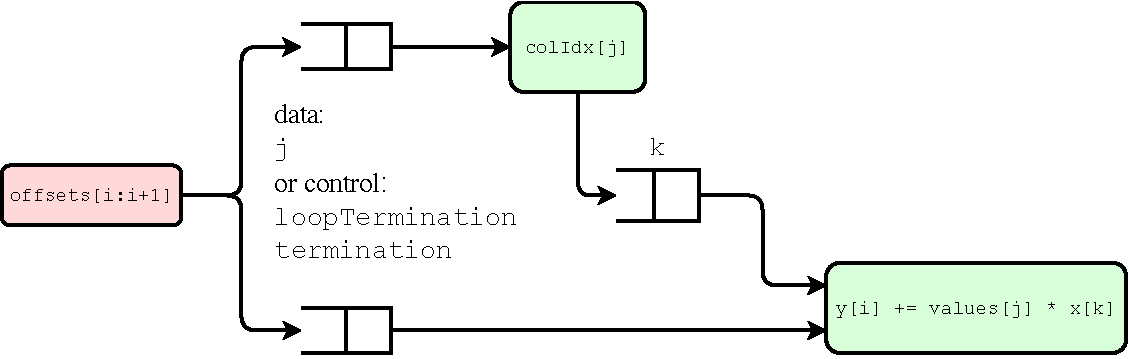
\includegraphics[width=0.5\textwidth,keepaspectratio]{spmv}

    %%%%%%%%%%%%%%%%%%%%%%%%%%%%%%%%%%%%%%%%%%%%%%%%%%%%%%%%%%%%%%%%%%%%%%%%%%%%%%%
    \section{Microarchitectural challenges}
    %%%%%%%%%%%%%%%%%%%%%%%%%%%%%%%%%%%%%%%%%%%%%%%%%%%%%%%%%%%%%%%%%%%%%%%%%%%%%%%
    The slicing requires ISA-visible queues, which should support:
    \begin{itemize}
    \item low-latency, fine-grained and blocking push/pop operations
    \item low-latency checks for control flow tokens
    \end{itemize}

    %%%%%%%%%%%%%%%%%%%%%%%%%%%%%%%%%%%%%%%%%%%%%%%%%%%%%%%%%%%%%%%%%%%%%%%%%%%%%%%
    \section{Related Work}
    %%%%%%%%%%%%%%%%%%%%%%%%%%%%%%%%%%%%%%%%%%%%%%%%%%%%%%%%%%%%%%%%%%%%%%%%%%%%%%%

    Manocha, A., Sorensen, T., Tureci, E., Matthews, O., Arag{\'{o}}n, J.L., and Martonosi, M. 2021.
    \textbf{GraphAttack: Optimizing Data Supply for Graph Applications on In-Order Multicore Architectures}
    ACM Transactions on Architecture and Code Optimization (TACO) 18, 1–26. \\

    Nguyen, Q.M. and Sanchez, D. 2023.
    \textbf{Phloem: Automatic Acceleration of Irregular Applications with Fine-Grain Pipeline Parallelism}
    2023 IEEE International Symposium on High-Performance Computer Architecture (HPCA).

  \end{multicols}
} % end of centerbox

%%%%%%%%%%%%%%%%%%%%%%%%%%%%%%%%%%%%%%%%%%%%%%%%%%%%%%%%%%%%%%%%%%%%%%%%%%%%%%%
\bottombox {
%%%%%%%%%%%%%%%%%%%%%%%%%%%%%%%%%%%%%%%%%%%%%%%%%%%%%%%%%%%%%%%%%%%%%%%%%%%%%%%
  \bottomboxlogo{university/chalmers_nologo_white}
  \hspace{8cm}  % hack for A0
  \bottomboxlogo[height=\bottomboxheight]{qr-dpref-waspblue}
  \hspace{-3cm} % hack for A0
  \bottomboxlogo{waspwhite}
}

\end{document}
